%---------- Inleiding ---------------------------------------------------------

\section{Introductie}%
\label{sec:introductie}
In het snel evoluerende domein van software-\\ontwikkeling wordt de behoefte aan flexibele en efficiënte tools om het ontwikkelingsproces te versnellen en te vereenvoudigen steeds \\belangrijker. Bij de introductie van de Swift \\OpenAPI Generator in juni, dacht men dat deze tool hiervoor een veelbelovende oplossing zou kunnen zijn. Dit onderzoek richt zich op de \\mogelijkheden van de Swift OpenAPI Generator, met specifieke focus op het vermogen om een werkend prototype te genereren en ook op hoe gemakkelijk het kan evolueren naar een \\productieklare back-end zonder een volledige herimplementatie. 

De doelstelling van dit onderzoek bestaat uit twee delen. Enderzijds richt het zich op het \\beoordelen van de capaciteiten van de Swift \\OpenAPI Generator. Anderzijds bestudeert het de haalbaarheid en efficiëntie van het evolueren van een prototype naar een productieklare back-end. 

Het concrete eindresultaat van dit onderzoek bestaat niet alleen uit een uitgeschreven \\scriptie, maar ook uit een tastbaar bewijs van de Swift OpenAPI Generator in actie. Het zal als een \\succesvolle bachelorproef beschouwd worden \\wanneer op een gemakkelijke manier een back-end kan gegenereerd worden die we als een \\productieklare back-end kunnen zien zonder dat er veel aanpassingen nog nodig zijn. Een \\rapport met aanbevelingen voor verdere \\optimalisatie en implementatie zou het sluitstuk kunnen vormen, waarbij het geheel als succesvol wordt beschouwd wanneer de Swift OpenAPI \\Generator daadwerkelijk bijdraagt aan het \\versnellen en vereenvoudigen van het \\ontwikkelingsproces.  

%---------- Stand van zaken ---------------------------------------------------

\section{Literatuurstudie}%
\label{sec:literatuurstudie}
De Swift OpenAPI Generator is een swift \\plugin, die code kan genereren die nodig is om API-oproepen te doen of API servers te \\implementeren. Het genereert de code aan de hand van de openAPI documenten. Dit zorgt ervoor dat Swift-ontwikkelaars snel en efficiënt clientcode kunnen genereren voor het gebruik van RESTfull API’s. Om de swift OpenAPI \\Generator te gebruiken moet je twee plugins toevoegen, de swift-openapi-generator en de swift-openapi-runtime. De eerste plugin genereert code tijdens build-time en de tweede plugin bevat \\protocol definities die worden gebruikt door de gegenereerde code en extensiebibliotheken.\\Hierna moet je nog 2 bestanden toevoegen aan uw project namelijk de openapi.yaml, beschrijft uw API, de openapi-generator-config.yaml is een configuratiebestand voor de plug-in die bepaalt of client- of servercode moet worden \\gegenereerd. Met zijn intuïtieve interface, \\uitgebreide functies en sterke community-\\ondersteuning is het een essentiële troef voor elke Swift-ontwikkelaar die met API's werkt \\ \autocite{Dvorsky2023} . 

De openAPI document is een open standaard voor het definiëren van HTTP APIs, meestal \\gedocumenteerd in YAML of JSON. OpenAPI-\\documenten zijn een essentieel hulpmiddel om consistentie en kwaliteit te waarborgen tijdens de ontwikkeling, doordat ze verschillende \\doeleinden dienen. De openAPI-documenten \\worden opgesteld volgens de OpenAPI-\\specificaties (OAS) en deze specificaties zorgen voor duidelijke, leesbare beschrijving van HTTP API’s voor zowel mensen als machines die het mogelijk maken een service te begrijpen zonder dat er veel kennis nodig is om met de service te communiceren \autocite{Miller2020}. 

Hoewel OpenAPI en Swagger verwant zijn, zijn ze niet identiek. OpenAPI vertegenwoordigt de evolutie van de Swagger 2.0-specificatie, die een nieuwe naam kreeg na de overname door SmartBear Software en de donatie aan het OpenAPI \\Initiative \autocite{2023}. OpenAPI is de specificatie die wordt gebruikt om RESTfull API's te definiëren. Swagger omvat een reeks tools die worden gebruikt om OpenAPI \\specification te implementeren. Swagger bevat ook een breed scala aan API-ontwerp-, \\documentatie-, test-, beheer- en monitoring-\\oplossingen die het voor ontwikkelaars \\gemakkelijker maken om de openAPI \\specificaties te implementeren \autocite{ Pinkham2017}. 

Een van de best practices om een API te \\ontwikkelen is om een API te creëren volgens de design principes van REST. Representational State Transfer is ontworpen om als richtlijn te \\dienen voor het beheren van communicatie \\binnen complexe netwerken zoals het internet. API’s die gebruik maken van REST worden REST API’s of RESTfull API’s genoemd. De principes van REST-architectuurstijl omvatten een uniforme \\interface, statelessness, een gelaagd systeem, \\cachebaarheid en code on demand. Door deze principes biedt Rest API verschillende voordelen, namelijk schaalbaarheid, flexibiliteit en \\onafhankelijkheid van specifieke technologieën. Dit betekent dat zowel client- als server-\\applicaties in verschillende programmeertalen \\kunnen worden geschreven zonder dat dit invloed heeft op het API-ontwerp \autocite{2020}. 

Het creëren van back-end in Swift wordt \\voornamelijk gedaan via Vapor. Het is een open-source web framework die geschreven is in Swift en is een krachtig framework voor het schrijven van web- en API-services \autocite{Nelson}. Vapor profiteert ook van het concurrency-model van Swift, deze maakt deelbare, veranderlijke status- en datarace-veiligheid mogelijk, waardoor een betrouwbaar en efficiënt framework kan worden aangeboden. Bovendien heeft Swift de laagste geheugen-\\voetafdruk van native gecompileerde binaire \\bestanden in Linux, waardoor Vapor een lichtgewicht en efficiënte keuze is. Het heeft een kleine leercurve voor native app-ontwikkelaars, waardoor het een go-to-oplossing is voor de \\ontwikkeling van API-services \autocite{Pant2023}.
% Voor literatuurverwijzingen zijn er twee belangrijke commando's:
% \autocite{KEY} => (Auteur, jaartal) Gebruik dit als de naam van de auteur
%   geen onderdeel is van de zin.
% \textcite{KEY} => Auteur (jaartal)  Gebruik dit als de auteursnaam wel een
%   functie heeft in de zin (bv. ``Uit onderzoek door Doll & Hill (1954) bleek
%   ...'')



%---------- Methodologie ------------------------------------------------------
\section{Methodologie}%
\label{sec:methodologie}

Voor het onderzoek naar de mogelijkheden van de Swift OpenAPI Generator is er een plan van aanpak. Dit plan van aanpak is opgedeeld in \\verschillende fases. 

In de eerste fase is het doel om een diepgaande kennis te verwerven over het onderwerp. Deze fase wordt opgedeeld in 3 deelfases. Als \\eerste richt men zich op de OpenAPI specificaties, omdat de Swift OpenAPI Generator sterk \\afhankelijk is van deze specificaties. Dit wordt gedaan om inzicht te krijgen over hoe OpenAPI wordt gebruikt in andere contexten om zicht te krijgen op de generieke bruikbaarheid van de OpenAPI specificaties. Naast het begrijpen van de OpenAPI specificaties, is het belangrijk dat er gekeken wordt naar de best practices en trends van de API-ontwikkeling en hoe back-ends \\doorgaans ontwikkeld en geoptimaliseerd \\worden. Hierna is van groot belang dat er \\gefocust wordt op het gebruik van Swift in Backend-ontwikkeling. 

Na deze eerste fase zullen er duidelijke doelstellingen worden bepaald voor het verder \\verloop van het onderzoek. Aan de hand van de \\literatuurstudie zullen deze doelstellingen \\worden vastgelegd om een duidelijk beeld te \\krijgen van wat de Swift OpenAPI Generator \\allemaal moet kunnen, namelijk is de Swift OpenAPI generator instaat om authentificatie of validatie toe te passen en API calls te beperken tot een \\specifieke rol. 

In de derde fase zullen er twee deelfases \\uitgewerkt worden. In de eerste deelfase zullen er \\mogelijk scenario's worden gecreëerd om de Swift OpenAPI-generator te testen. Er zullen vijf \\verschillende scenario's worden uitgewerkt, waarbij elke keer een iets complexere API nodig zal zijn. Hierbij zullen de OpenAPI-specificaties en de literatuurstudie worden gebruikt om de \\mogelijke scenario's uit te werken. Nadat deze scenario’s zijn uitgeschreven kan er werk gemaakt worden van de tweede deelfase. In de volgende fase zal een Swift UI uitgewerkt worden waarbij je gemakkelijk kan zien hoe deze API’s werken. Deze Swift UI zal gebruikt worden om na te gaan of het mogelijk is om een snelwerkend prototype te creëren. 

In de volgende fase zullen alle mogelijke \\scenario’s worden uitgewerkt met de Swift OpenAPI Generator. Ook zullen ze getest worden met de Swift UI die gecreëerd is in de voorgaande fase. Deze fase wordt gedaan om te weten te komen hoe gemakkelijk het is om een werkend \\prototype te genereren. 

Na deze fase zullen de verzamelde gegevens geanalyseerd worden om inzicht te krijgen in de prestaties van de Swift OpenAPI Generator. Ook zullen de gegevens met elkaar worden \\vergeleken en zal het meest effectieve scenario \\worden geïdentificeerd aan de hand van de vooraf bepaalde doelstellingen. Ook zullen de \\eventuele beperkingen van de Swift OpenAPI \\Generator worden geïdentificeerd.

Als laatste zal er een conclusie worden \\getrokken uit het onderzoek en een antwoord worden geformuleerd op de onderzoeksvraag op basis van de verkregen resultaten. Ook zal er een aanbeveling worden geschreven voor het gebruik van de Swift OpenAPI generator. 

\begin{center}
    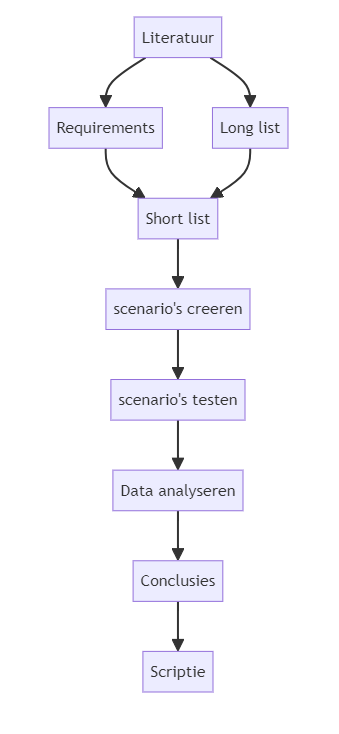
\includegraphics[scale=0.6]{methodologie.png}
\end{center}

%---------- Verwachte resultaten ----------------------------------------------
\section{Verwacht resultaat, conclusie}%
\label{sec:verwachte_resultaten}

Aan de hand van mijn literatuurstudie kan er afgeleid worden dat de Swift OpenAPI generator goed zal werken bij gemakkelijkere API’s, maar minder goed bij complexere API’s. Bij voorgaande tools die code genereren is het vaak zo dat er nog veel zaken moeten aangepast worden, maar \\wanneer je dit opnieuw laat genereren ben je je aanpassingen weer kwijt en moet je weer \\opnieuw beginnen. Zelf hoop ik dat ik deze \\verwachtingen kan weerleggen, zou het een zeer nuttig instrument kunnen zijn voor het ontwikkelen van een back-end. Dit zou ervoor zorgen dat de developers meer tijd kunnen besteden aan de apps interface. 